\section{Background}
\label{background}
This section will present relevant background information for reading this paper, including the research area in section \ref{research_area}, the \qs{} algorithm in \ref{qs}, and related work in \ref{state_of_the_art}.

\subsection{Research area}
\label{research_area}
%What is the research area?
Various applications of algorithms to find distances between data points in a (typically large) data set exist. One example is doing similarity search, or more specifically nearest-neighbor (NN) search, on images to recognize letters or numbers. While useful, it is quite data dependent and suffer from the \textit{curse of dimensionality}\footnote{See \url{https://en.wikipedia.org/wiki/Curse_of_dimensionality} for information on this property}. This is a general problem as even modern machines are not able to process \textit{gigantic} files(i.e. keeping all the data in main memory). Thus another big subject in computer science arises, that is compressing the data in order to fit it in memory while trying to preserve as many properties from the data as possible. This research area, in particular for high-dimensional data setsm is what \qs{} deals with.
\\
\\
Naturally one must pay to compress something, which happens in terms of accuracy, i.e. representing the data using only approximations. This also means there is a trade off between compression and accuracy for the algorithms in this area. That is why compression algorithms usually are measured on these parameters, i.e. accuracy per compression size.
\\
\\
Distance preserving compression algorithms are usually divided into two categories: data-oblivious and data-dependent. The former attempts to achieve guarantees for any data set while the latter attempts to use the extra information about the particular data sets in order to design functions with better performance. Compressed representations makes computation for data analysis algorithms more efficient, which is very desirable in many fields, such as data mining and machine learning\cite{stan15}.

\subsection{The \qs{} compression scheme}
\label{qs}
In this sections the \qs{} algorithm is outlined. The compression scheme that it comprises produces a sketch, which is a compressed representation of a point set \texttt{X}. The points of \texttt{X} have \texttt{d} dimensions and are in \textit{Euclidean} space. Each coordinate of a point is represented by \texttt{B} bits implying that a point is represented by \textit{dB} bits. \qs{} require the point set \texttt{X} and two additional parameters, namely \texttt{L} and $\Lambda$ as input. These two parameters are used to specify the compression of the point set where \texttt{L} is the depth of the \qt{} and $\Lambda$ controls amount of nodes from \qt{} which can be pruned. 

There are three steps for building the sketch: randomly shifted grid, \qt{} construction and pruning. These steps will be explained briefly and there will be given an example of how a sketch is built on a small example.
\\
\\
The first step is to produce a randomly shifted grid on the hypercube(an n-dimensional space) \texttt{H} which contains all points of the given point set \texttt{X}. \texttt{H} will then be set up to be centered around a point of \texttt{X}. Then choose a random value $\sigma_j$ for each dimension \texttt{j} to shift \texttt{H}. This results in a randomly shifted axis-parallel grid on the points. It is however noted in the paper that this step often can be eliminated in practice without affecting the empirical performance of the algorithm, but that is is necessary for achieving guarantees for arbitrary point sets\cite[p. 4, "Step 1[..]"]{wagner17}.
\\
\\
The next step is to create the \qt{}. A \textit{2d-ary} \qt{} is created by starting at the root of \texttt{H}. Child nodes are only added for the corresponding grid cells that contain at least one point of \texttt{X}, and thus child nodes that do not contain a point from \texttt{X} are ignored. Each edge to a child node is labeled with a \textit{d} long bit string that has been split on. This step is done recursively until the level \texttt{L} is reached. An example of a constructed \qt{} is given in figure \ref{fig:quadtree}.

\begin{figure}
	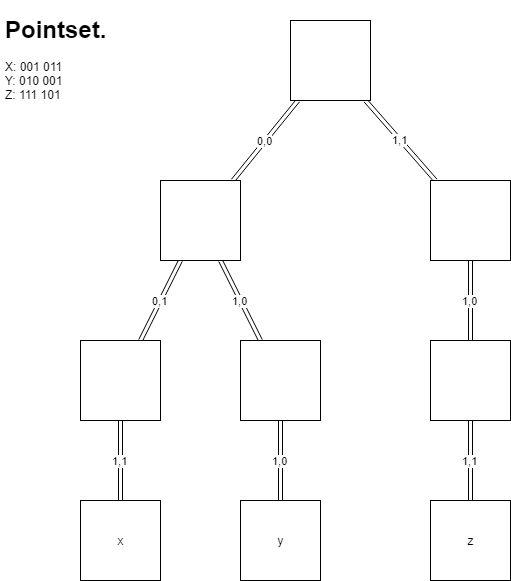
\includegraphics[width=0.5\textwidth]{figures/quadtree}
	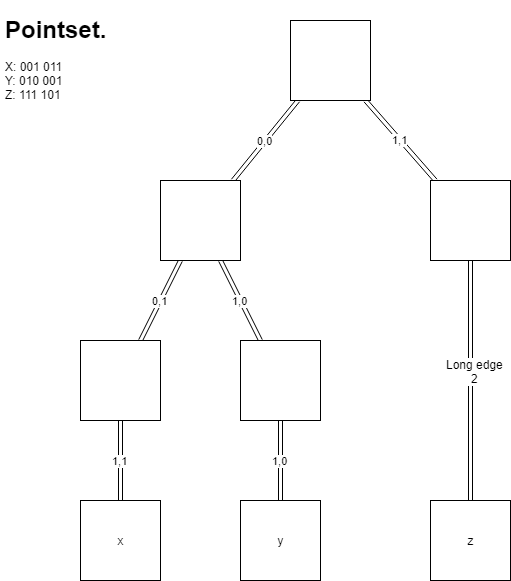
\includegraphics[width=0.5\textwidth]{figures/prunnedquadtree}
	\caption{On the left there is shown the \qt{} after construction with $L=4$. On the right the \qt{} has been pruned with a $\Lambda = 1$}
	\label{fig:quadtree}
\end{figure}

The final step is the pruning. For each downward path $n_0,...,n_k$ in the \qt{} where nodes $n_1,...,n_{k-1}$ all have a degree 1, if \ensuremath{\texttt{k} > \Lambda+1} then corresponding nodes $n_{\Lambda+1},...,n_{k-1}$ are removed from the \qt{}. Instead node $n_{\Lambda}$ is connected directly to $n_{k}$ with an edge. This edge is called a \textit{long edge} and is labeled with the length of the path it replaces. An example of the tree after a pruning is given in figure \ref{fig:quadtree}.


To represent the sketch the "Eulerian Tour Technique"\footnote{See e.g., \url{https://en.wikipedia.org/wiki/Euler\_tour\_technique}} is used.
It starts at the root of the tree and searches down to the leftmost leaf. It will then backtrack up to a node from which it can again traverse down to find a new leaf. When an edge is explored downwards a 0 is stored and the label of the edge, being either a bit string or the length of a long edge. Also for each downward movement a bit specifying if the given edge is a long or short edge is stored. If an upwards edge is explored a 1 is stored. Furthermore, there is stored an index for each point for the child node which contains it.
%TODO: Review this subsection to properly and precisely describe QS

%From ILO:
%"Find, extract and explain results in the algorithms research literature relevant to a given problem."
\subsection{Related work}
\label{state_of_the_art}
Several state of the art algorithms exist for the research area introduced in section \ref{research_area}. \cite{wagner17} mentions \textit{Product Quantization} (\pq{}), which they use as reference state of the art algorithm in their experiments. The \pq{} concept is stated in its original paper, \cite{schmid9}, as such "The idea is to decomposes the space into a Cartesian product of low dimensional subspaces and to quantize each subspace separately", where the term \textit{quantize} refers to the process of constraining an input from a continuous set of values to a discrete set\footnote{E.g. real numbers to integers. See https://en.wikipedia.org/wiki/Quantization 11-04-2018}.

Well known general algorithms and data structures exists for the same purpose, such as \textit{k-means} and \textit{kd-trees}, where the former is a clustering algorithm and the latter is an adaptive data structure for spatial data sets. This is also discussed in \cite{schmid9}, where it is noted that apparently a pure brute-force algorithm outperforms these in practice for high-dimensional data. Further algorithms listed in this paper include "spectral hashing"\cite{weiss8}, "Hamming embedding"\cite{jegou8}, and "FLANN"\cite{muja9}. These will not be investigated further, but are only mentioned for reference.
%TODO: Elaborate on closely related work and insert citations